\documentclass[11pt]{article}
\usepackage[margin=24mm]{geometry}
\usepackage[T1]{fontenc}
\usepackage{lmodern}
\usepackage{microtype}
\usepackage{amsmath,amssymb,mathtools}
\usepackage{booktabs,tabularx,array,multirow}
\usepackage{float}
\usepackage{enumitem}
\usepackage{xcolor}
\usepackage{graphicx}
\usepackage{tikz}
\usetikzlibrary{arrows.meta,positioning,fit,shapes.geometric}
\usepackage{pgfplots}
\pgfplotsset{compat=1.18}
\usepgfplotslibrary{dateplot}
\usepackage{hyperref}
\usepackage{xurl}

\definecolor{ink}{HTML}{17212B}
\definecolor{navy}{HTML}{183B56}
\definecolor{teal}{HTML}{0B7A75}
\definecolor{amber}{HTML}{B7791F}
\definecolor{red}{HTML}{B42318}
\definecolor{pale}{HTML}{F3F7F9}
\definecolor{grid}{HTML}{D7E1E7}

\hypersetup{
  colorlinks=true,
  linkcolor=navy,
  citecolor=teal,
  urlcolor=navy,
  pdftitle={From Backtest to Public Record: A Fail-Closed Evidence Architecture for Prospective Validation of Systematic Trading Systems},
  pdfauthor={Arhan Canli},
  pdfsubject={Prospective validation, quantitative finance, reproducible research},
  pdfkeywords={systematic trading, prospective validation, reproducibility, provenance, paper trading, transparency log}
}

\setlist{nosep,leftmargin=*}
\setlength{\parindent}{0pt}
\setlength{\parskip}{0.55em}
\renewcommand{\arraystretch}{1.16}

\newcommand{\system}{\textsc{Alphac}}
\newcommand{\code}[1]{\texttt{#1}}
\newcommand{\status}[1]{\texttt{#1}}
\newcommand{\evidence}{\textsc{evidence}}
\newcommand{\simulation}{\textsc{simulation}}
\newcommand{\planned}{\textsc{planned}}

\title{\vspace{-1.4em}\textbf{From Backtest to Public Record}\\[0.35em]
\Large A Fail-Closed Evidence Architecture for Prospective Validation of Systematic Trading Systems}
\author{Arhan Canli\\Independent Researcher, United Arab Emirates\\\href{https://canlicapital.com}{canlicapital.com}}
\date{26 August 2026\\Author-review draft v0.1.0; not submitted; not peer reviewed}

\begin{document}
\maketitle

\begin{center}
\fcolorbox{grid}{pale}{\parbox{0.92\linewidth}{\raggedright
\textbf{Claim boundary.} The empirical material in this paper is self-published paper-trading and research-simulation evidence. It is not funded performance, an independent broker attestation, a statistically established Sharpe ratio, or evidence of future returns. The case-study record contains 17 daily return observations as of 26 August 2026 and is deliberately classified as immature.
}}
\end{center}

\begin{abstract}
Backtest overfitting is usually treated as a statistical problem. In a deployed research programme it is also a systems problem: a reported result is difficult to interpret when the tested identity, data vintage, runtime configuration, execution record, and publication state can change independently. This paper presents a fail-closed evidence architecture for prospective validation of systematic trading systems. The design binds each research trial to a canonical identity before result inspection; fingerprints the live configuration by evidence epoch; reconciles paper execution against read-only broker records; commits public evidence to a signed, append-only hash chain; and evaluates performance claims through an explicit maturity state machine. A claim is suppressed whenever any mandatory provenance predicate fails, even if the underlying return statistic is favorable.

We evaluate the architecture through the
\system{} implementation and a dated case-study snapshot. At the snapshot, 44 provenance predicates pass, three dedicated Alpaca paper accounts reconcile, and all 48 publication guards fail under their intended semantic mutations while one inert negative control survives. The public chain contains 502 signed entries, of which 66 disclose canonical payloads; the earlier 436 entries remain opaque commitments and cannot be reconstructed from the public record. Most importantly, the architecture refuses to publish a mature Sharpe estimate from 17 daily returns. The paper record is down 2.46\%, with 2.57\% realized maximum drawdown. A separate current-composition model estimates 9.32\% expected maximum drawdown and 16.45\% at the 95th percentile, but neither quantity is treated as live establishment. The contribution is not a profitable strategy claim. It is an executable method for making the distance between a backtest, a paper record, and an established performance claim explicit and auditable.
\end{abstract}

\textbf{Keywords:} systematic trading; prospective validation; reproducible research; provenance; paper trading; transparency logs; backtest overfitting

\section{Introduction}

The weakest point in a systematic strategy is often not its optimizer. It is the boundary between what was tested, what was deployed, and what was later claimed. A backtest can be corrected for non-normality and selection bias yet remain unconvincing if the number of attempted specifications is unknown, the production configuration is not identifiable, or the public performance curve can be replaced without a visible discontinuity. Conversely, a cryptographically signed record can preserve an incorrect number perfectly. Statistical validity, computational reproducibility, execution provenance, and publication integrity solve different failure modes.

The quantitative-finance literature provides strong tools for data snooping, multiple testing, and uncertainty in risk-adjusted performance \cite{white2000reality,lo2002statistics,bailey2014deflated,bailey2017pbo,harvey2016crosssection}. Reproducible-computing guidance emphasizes executable workflows, exact software versions, and retained intermediate evidence \cite{sandve2013ten}. Provenance standards represent how entities, activities, and agents produce a result \cite{w3c2013prov}. Transparency-log protocols show how signed append-only structures can make later mutation detectable \cite{laurie2021ct}. These ideas are individually mature. They are rarely composed into one operational claim system for a continuously running strategy.

This paper asks a practical question:

\begin{quote}
What must a trading-research system preserve so that a skeptical reader can distinguish a historical simulation, a prospective paper observation, and a statistically established performance claim without trusting the publisher's interface?
\end{quote}

We answer with an architecture organized around four invariants:

\begin{enumerate}
  \item \textbf{Identity before outcome.} A trial is named by its economic and computational choices before its return-bearing result is inspected.
  \item \textbf{Configuration continuity.} A live record belongs to a fingerprinted evidence epoch; material configuration changes start a new epoch instead of silently extending the old one.
  \item \textbf{Fail-closed claims.} Performance maturity is the conjunction of statistical and provenance conditions. A broken input suppresses the stronger claim.
  \item \textbf{Publicly testable publication.} Published artifacts carry content hashes, source bindings, machine-readable status, and mutation-tested guards.
\end{enumerate}

The contribution is the composition and operationalization of these invariants. We do not claim that hashing, digital signatures, broker reconciliation, preregistration, or Sharpe-ratio corrections are new. We contribute a domain-specific evidence graph, a claim-maturity state machine, and an implementation evaluation that makes their interactions explicit.

\section{Related work and unresolved gap}

\subsection{Selection bias and risk-adjusted performance}

White's Reality Check formalizes inference after specification search \cite{white2000reality}; Hansen's test improves power when many poor alternatives are present \cite{hansen2005spa}. Bailey and L\'opez de Prado develop probabilistic and deflated Sharpe-ratio methods that account for finite samples, non-normality, and selection effects \cite{bailey2012sharpe,bailey2014deflated}. Bailey et al. propose combinatorially symmetric cross-validation to estimate the probability of backtest overfitting \cite{bailey2017pbo}. Harvey, Liu, and Zhu show why ordinary significance thresholds become inadequate when the effective factor search is large \cite{harvey2016crosssection}.

These methods address inference conditional on an identified search and return matrix. An operational programme must first answer what counts as a trial, whether identities were omitted, which configuration generated the live record, and whether the displayed series is the one evaluated. The architecture below treats those questions as machine-enforced prerequisites rather than narrative footnotes.

\subsection{Reproducibility and provenance}

Reproducible computational research requires the exact workflow, inputs, parameters, and software versions that produced a result \cite{sandve2013ten}. The W3C PROV family distinguishes entities, activities, and agents so provenance can be represented and exchanged \cite{w3c2013prov}. These principles motivate the evidence graph in Section~\ref{sec:graph}, but a financial deployment adds two complications. First, some vendor inputs cannot be redistributed. Second, the result-generating system continues to change after publication. Hash-only bindings can identify restricted inputs without granting access, while evidence epochs prevent changed production logic from inheriting an earlier track record.

\subsection{Append-only transparency}

Merkle trees and signed log heads support efficient detection of inconsistent or rewritten histories \cite{merkle1988digital,laurie2021ct}. A trading evidence log has a narrower goal than Certificate Transparency: it commits to published state transitions and makes mutation detectable. It does not prove that a broker, data vendor, or publisher told the truth. It also cannot prove completeness when an event was never logged. Our threat model therefore treats cryptographic integrity as one predicate among many, not as a substitute for economic or statistical verification.

\subsection{Trading-system verification}

Existing trading frameworks connect strategy development, backtesting, paper testing, and production execution \cite{decastro2021mt5se}. Work on backtest-engine correctness shows that apparently simple historical execution rules require explicit models and targeted verification cases \cite{low2015correctness}. These systems motivate treating implementation as part of research validity. Our scope is complementary: we do not propose a new execution simulator or trading-agent architecture. We govern the identity and maturity of claims as they move from a research search to a changing paper deployment and then to a public record.

\section{System model and threat model}

The system has four actors: a researcher who specifies and evaluates trials; an execution service that runs a paper portfolio; external data and broker services; and a public reader who may not trust the publisher. A single person may operate the first two roles. No independence is inferred from role separation inside one project.

We consider six failure classes:

\begin{enumerate}
  \item \textbf{Search omission:} losing or merging unsuccessful trial identities so the apparent search is smaller than the real search.
  \item \textbf{Temporal leakage:} using revised, late, or future-known data in a historical decision.
  \item \textbf{Configuration drift:} changing live logic while reporting one uninterrupted record.
  \item \textbf{Execution substitution:} presenting simulated fills or local marks as broker-derived observations without a visible boundary.
  \item \textbf{Publication mutation:} changing a result, status, or historical curve after publication without a new version.
  \item \textbf{Claim escalation:} presenting an immature point estimate, a model output, or a paper account as established or funded performance.
\end{enumerate}

The design assumes that the operator may make mistakes and may face incentives to present favorable evidence. It does not assume compromise of SHA-256 or Ed25519. It does assume that the operator controls the signing key; therefore a valid signature proves key authorization, not author identity or truth. Split-view logs, omitted events, collusion with upstream providers, and fabricated source data remain outside the guarantee unless independently monitored.

\section{Evidence architecture}
\label{sec:graph}

\subsection{Canonical evidence graph}

Each public claim is a node in a directed acyclic evidence graph. A node contains a schema identifier, canonical payload, content hash, status token, claim boundary, and bindings to its immediate authorities. Edges are typed: \emph{derived from}, \emph{configured by}, \emph{executed as}, \emph{reconciled against}, or \emph{published as}. The graph is valid only when every required node exists, rehashes to its declared digest, and satisfies its schema-specific predicate.

Let $x_i$ be a canonicalized evidence object and
\begin{equation}
  d_i = H(\operatorname{canon}(x_i)),
\end{equation}
where $H$ is SHA-256. A claim object $y$ binds its direct authorities by path and digest:
\begin{equation}
  y.\mathrm{sources} = \{(p_i,d_i)\}_{i=1}^{m}.
\end{equation}
Reproduction means more than recomputing $d_i$. A verifier re-evaluates the transformation from authorities to claim and compares the canonical output. The hash detects changed bytes; the replay tests the stated computation.

\begin{figure}[H]
\centering
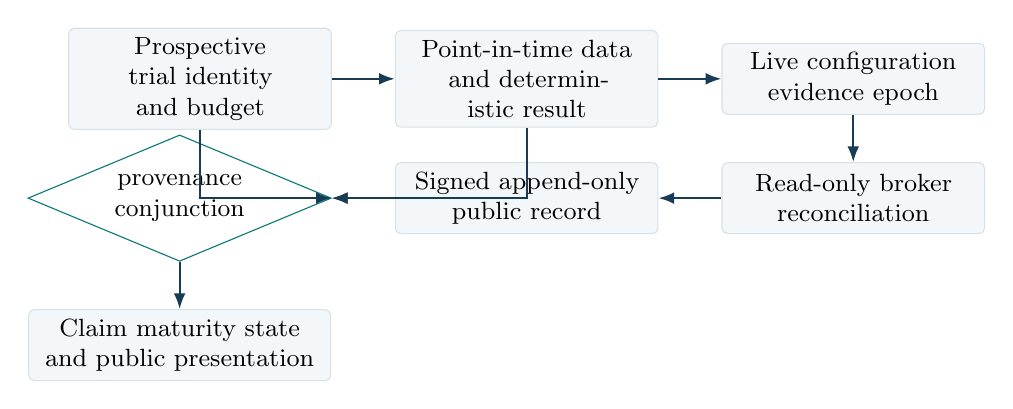
\begin{tikzpicture}[
  node distance=6mm and 8mm,
  box/.style={draw=grid,rounded corners=2pt,fill=pale,minimum height=9mm,text width=31mm,align=center,font=\small},
  gate/.style={draw=teal,diamond,aspect=2.4,fill=white,align=center,font=\small},
  arrow/.style={-{Latex[length=2mm]},thick,draw=navy}
]
\node[box] (identity) {Prospective trial identity\\and budget};
\node[box,right=of identity] (result) {Point-in-time data\\and deterministic result};
\node[box,right=of result] (config) {Live configuration\\evidence epoch};
\node[box,below=of config] (broker) {Read-only broker\\reconciliation};
\node[box,left=of broker] (chain) {Signed append-only\\public record};
\node[gate,left=of chain] (gate) {provenance\\conjunction};
\node[box,below=of gate,text width=36mm] (claim) {Claim maturity state\\and public presentation};
\draw[arrow] (identity) -- (result);
\draw[arrow] (result) -- (config);
\draw[arrow] (config) -- (broker);
\draw[arrow] (broker) -- (chain);
\draw[arrow] (chain) -- (gate);
\draw[arrow] (identity) |- (gate);
\draw[arrow] (result) |- (gate);
\draw[arrow] (gate) -- (claim);
\end{tikzpicture}
\caption{The claim is downstream of both the statistical result and its provenance. A favorable return cannot bypass a failed identity, configuration, broker, continuity, or publication predicate.}
\label{fig:architecture}
\end{figure}

\subsection{Prospective trial identity}

A trial identity is not a filename or a row number. It is a digest of choices that can change the economic hypothesis or measured outcome:
\begin{equation}
  \tau = H(f,u,d,v,\theta,c,o,s),
\end{equation}
where $f$ is the hypothesis family, $u$ the universe, $d$ the data definition, $v$ the vintage and availability rule, $\theta$ the parameterization, $c$ the cost and execution model, $o$ the objective, and $s$ the sample partition. Economically identical identities may be deduplicated only under a declared equivalence rule. Rounded summary statistics are never sufficient evidence of identity equivalence.

The ledger has a prospective budget. Registering an identity consumes budget before return-bearing data are opened. Budget exhaustion pauses new trials; it does not relax the gate or authorize a successful label. Historical studies discovered outside the durable ledger are charged as trial debt and remain marked as reconstructed rather than prospectively registered.

\subsection{Evidence epochs and configuration fingerprints}

For live epoch $e$, the system derives
\begin{equation}
  \lambda_e = H(\operatorname{canon}(C_e)),
\end{equation}
where $C_e$ includes every setting that changes portfolio decisions, sizing, overlays, and aggregation. The published state declares $\lambda_e$, and the evaluator independently derives it from runtime defaults and configuration. A mismatch fails the provenance gate. A material change creates epoch $e+1$ and resets the forward performance claim unless a predeclared rule explicitly preserves admissible observations.

This rule prevents a common ambiguity: a curve may be continuous in date while discontinuous in specification. The architecture gives specification continuity priority over visual continuity.

\subsection{Broker-derived paper evidence}

Paper execution is reconciled through read-only broker endpoints for account state, positions, portfolio history, and open orders. For account $a$ and timestamp $t$, local equity $E^{L}_{a,t}$ and broker equity $E^{B}_{a,t}$ must agree within a declared currency tolerance:
\begin{equation}
  |E^{L}_{a,t} - E^{B}_{a,t}| \leq \epsilon.
\end{equation}
The reconciliation also checks paper endpoint, account status, account uniqueness, nontrivial history, mark coverage, fill-reconciliation health, freshness, and temporal coverage of the published state.

Broker-derived does not mean independently attested. The operator selects the API query, transforms the response, and publishes the receipt. The evidence is stronger than a locally generated fill model because it can be checked against a distinct service, but it remains self-published and paper-only.

\subsection{Signed append-only public record}

For public entry $t$, let $p_t$ be the canonical payload, $h_t=H(p_t)$ its digest, and $z_{t-1}$ the preceding chain hash. The implementation computes
\begin{equation}
  z_t = H(t \parallel q_t \parallel h_t \parallel z_{t-1})
\end{equation}
for sequence number $t$ and timestamp $q_t$, then publishes an Ed25519 signature $\sigma_t=\operatorname{Sign}_{sk}(z_t)$ \cite{josefsson2017eddsa}. A verifier checks sequence continuity, predecessor hashes, payload hashes where payloads are disclosed, and signatures.

This is a linear signed hash chain, not a Certificate Transparency implementation. The comparison to transparency logs is conceptual: both make inconsistent history detectable under stated observation assumptions. Selected chain heads may receive external timestamp evidence, but timestamps do not validate the payload and are not required for the maturity evaluator.

\subsection{Fail-closed claim maturity}

Let $P_j \in \{0,1\}$ denote mandatory provenance predicates and
\begin{equation}
  G = \bigwedge_{j=1}^{k} P_j.
\end{equation}
The maturity function $M(R,C,G)$ maps return evidence $R$, a frozen claim contract $C$, and provenance conjunction $G$ to one public state. If $G=0$, the output is \status{FAIL\_CLOSED\_PROVENANCE} regardless of the statistic.

The current contract uses four statistical states:

\begin{table}[H]
\centering
\small
\begin{tabularx}{\linewidth}{>{\raggedright\arraybackslash}p{35mm}>{\raggedright\arraybackslash}p{36mm}X}
\toprule
State & Minimum condition & Permitted interpretation \\
\midrule
\status{IMMATURE} & $T<252$ daily returns & Cumulative return and realized drawdown may be shown; no mature Sharpe estimate. \\
\status{ESTIMATE} & $T\geq252$ & A point estimate and uncertainty measure may be shown. \\
\status{OBSERVED} & Point Sharpe $\geq1.5$ & The sample crossed the target, but establishment conditions are incomplete. \\
\status{ESTABLISHED} & $T\geq756$, point Sharpe $\geq1.5$, and $\Pr(SR>1.5)\geq0.95$ & The paper record establishes the target under this contract, subject to its paper-capital boundary. \\
\bottomrule
\end{tabularx}
\caption{Project-specific maturity contract. The sample thresholds are governance choices, not proposed universal constants.}
\label{tab:maturity}
\end{table}

The probability calculation uses the non-normal Probabilistic Sharpe Ratio. For per-period Sharpe $\widehat{SR}$, sample skewness $\widehat{\gamma}_3$, non-excess kurtosis $\widehat{\gamma}_4$, benchmark $SR^*$, and $T$ returns,
\begin{equation}
 \operatorname{PSR}(SR^*) = \Phi\!\left(
 \frac{(\widehat{SR}-SR^*)\sqrt{T-1}}
 {\sqrt{1-\widehat{\gamma}_3\widehat{SR}+\frac{\widehat{\gamma}_4-1}{4}\widehat{SR}^{2}}}
 \right).
\end{equation}
The annual target is converted to the return frequency before evaluation. Annualization changes units, not information. The full research search is separately charged through trial accounting and deflated-Sharpe diagnostics; the forward maturity test does not erase that historical search.

\subsection{Three drawdown claims}

The architecture distinguishes:

\begin{enumerate}
  \item realized maximum drawdown in the observed paper curve;
  \item modeled expected maximum drawdown under a named simulation design; and
  \item a tail statistic, currently the 95th percentile of modeled maximum drawdown.
\end{enumerate}

These quantities answer different questions. A short realized drawdown is descriptive. A modeled expectation depends on production equivalence and regime coverage. A tail estimate can exceed an expected-drawdown objective even when the expectation is inside it. The public claim must preserve all three labels.

\section{Implementation}

The reference implementation, \system{}, is a Python research and paper-execution system. Its publication layer exports machine-readable JSON to two public hosts and a human-readable evidence interface. The evaluator reads twelve authorities: forward contract, paper state, continuity audit, broker reconciliation, two drawdown studies, diversification study, sealed drawdown-evidence object, public transparency chain, crypto position attribution, rollout verification, and the methodology specification. Each output carries source bindings and a canonical content hash.

The central evaluator follows the procedure below.

\begin{center}
\fcolorbox{grid}{pale}{\parbox{0.92\linewidth}{\raggedright
\textbf{Fail-closed evaluation procedure}

1. Parse the flagship curve; reject duplicate dates, non-finite equity, or non-positive equity.\\
2. Derive returns without inserting synthetic zero-return dates.\\
3. Rehash every bound evidence object and validate its schema.\\
4. Recompute the live configuration fingerprint and check evidence-epoch continuity.\\
5. Validate record continuity, broker freshness, account uniqueness, and cent-level overlapping marks.\\
6. Validate the signed chain and require its disclosed head payload to equal the canonical state.\\
7. Recompute position arithmetic and account-equity reconciliation for the local crypto paper sleeve.\\
8. Evaluate Sharpe maturity and drawdown labels.\\
9. If any mandatory provenance predicate fails, replace the statistical state with \status{FAIL\_CLOSED\_PROVENANCE}.\\
10. Emit a canonical, content-hashed maturity object and publish identical bytes to both hosts.
}}
\end{center}

Publication guards test more than clean execution. A semantic mutation ledger changes one governed claim or authority at a time, executes the guard, records whether the mutation was caught, and verifies byte-identical restoration. A negative control edits a comment that should not affect behavior. This prevents an always-failing harness from appearing perfectly sensitive.

\section{Evaluation}

\subsection{Questions and frozen snapshot}

The evaluation addresses four questions:

\begin{description}[style=nextline]
  \item[RQ1: Integrity sensitivity.] Do publication guards fail when their governed semantics are mutated?
  \item[RQ2: Premature-claim suppression.] Does the maturity evaluator withhold a Sharpe estimate from an immature record?
  \item[RQ3: Execution provenance.] Can local paper state be reconciled to dedicated broker paper accounts without write access?
  \item[RQ4: Boundary visibility.] Does the public record expose negative outcomes and limitations rather than only successful checks?
\end{description}

The case-study snapshot is frozen at source commit \code{0b0ae0c12e042f20a9fff06d83255274804a3619} for the research engine and commit \code{9da32baf2bb75a76faca684e31034f2d5d1f7924} for the public site. The accompanying \path{case_study_snapshot.json} records exact SHA-256 source bindings. No result-bearing historical trial is opened or rerun for this paper.

\subsection{Integrity sensitivity}

The mutation ledger derives its guard set from tests over published claims. At the snapshot, 48 of 48 guards were mutated. Every intended semantic mutation was caught, every target was restored byte-identically, and the one inert negative control survived. Example mutations include corrupting the live-configuration fingerprint, publishing a stale contract, relabeling chain entries as days, breaking cross-profile trial deduplication, changing a public bundle byte, and forcing a lineage audit to pass unconditionally.

This is evidence that each listed guard can fail under one designed fault. It is not exhaustive mutation coverage of the codebase, proof of program correctness, or independent replication. The mutations were designed and run inside the project.

\subsection{Current evidence state}

\begin{table}[H]
\centering
\small
\begin{tabularx}{\linewidth}{>{\raggedright\arraybackslash}p{42mm}>{\raggedright\arraybackslash}p{38mm}X}
\toprule
Measure & Snapshot value & Interpretation \\
\midrule
Capital boundary & Paper only & No funded performance is in the published record. \\
Forward period & 7--26 Aug. 2026 & 18 marks and 17 daily return observations. \\
Cumulative return & $-2.4605\%$ & Observed paper result; no annualized inference. \\
Realized maximum drawdown & $2.5657\%$ & Descriptive to date, not expected maximum drawdown. \\
Sharpe maturity & \status{IMMATURE} & 235 observations remain before the 252-return estimate floor. \\
Provenance gate & 44 of 44 predicates pass & Internal source-bound validation, not independent attestation. \\
Broker reconciliation & 3 of 3 paper accounts pass & Read-only Alpaca evidence; unique dedicated accounts. \\
Public chain & 502 signed entries & 66 disclosed payloads; 436 earlier opaque commitments. \\
Sleeve state & 4 current; 14 target & The target is a research objective, not an achieved count. \\
\bottomrule
\end{tabularx}
\caption{Observed case-study state as of 26 August 2026.}
\label{tab:snapshot}
\end{table}

Figure~\ref{fig:curve} shows the complete normalized composite marks used by the maturity evaluator. The decline is retained because an evidence system is most informative when it publishes an unfavorable early path without changing the specification or suppressing the record.

\begin{figure}[H]
\centering
\begin{tikzpicture}
\begin{axis}[
  width=0.94\linewidth,
  height=58mm,
  date coordinates in=x,
  xticklabel style={rotate=35,anchor=east,font=\small},
  yticklabel style={font=\small},
  xlabel={UTC mark date},
  ylabel={Normalized paper equity},
  ymin=97.2,
  ymax=100.4,
  grid=both,
  major grid style={draw=grid},
  minor grid style={draw=grid!45},
  axis line style={draw=ink},
  tick style={draw=ink},
  line width=0.9pt
]
\addplot[teal,very thick,mark=*,mark size=1.5pt] table[x=date,y=equity,col sep=comma] {case_study_equity.csv};
\addplot[red,dashed,thick] coordinates {(2026-08-07,100) (2026-08-26,100)};
\end{axis}
\end{tikzpicture}
\caption{Complete normalized paper composite in the frozen snapshot. The dashed line is the starting level, not a benchmark return series.}
\label{fig:curve}
\end{figure}

The maturity evaluator returns \status{IMMATURE\_RECORD\_TOO\_SHORT}. It publishes no annualized point Sharpe and no probability that true Sharpe exceeds the 1.5 target. This answers RQ2 affirmatively: the public statistic is suppressed even though it is computationally possible to annualize 17 returns.

\subsection{Broker reconciliation}

Three dedicated Alpaca paper accounts pass the reconciliation procedure. Across the snapshot they contain 193 open positions and 149 open orders. Every overlapping broker portfolio-history mark matches local persisted history to the cent after refresh, the paper endpoint and active status checks pass, and the accounts are distinct. The fourth sleeve is a locally simulated crypto paper account and is governed by separate position-attribution and arithmetic checks.

The counts are operational state, not measures of strategy quality. Open-order counts are especially transient. The useful result is that the paper-performance provenance gate is tied to fresh broker-derived evidence and fails if that evidence becomes stale or inconsistent.

\subsection{Drawdown and diversification boundaries}

The current-composition simulation estimates expected maximum drawdown of 9.32\%, inside the 11\% objective, while its modeled 95th percentile is 16.45\%, outside that objective. Production equivalence is not established because the common history omits the COVID-19 and 2022 regimes, the block bootstrap cannot invent absent crises, the stress model lacks a volatility multiplier, and the study does not replay instrument-level execution gaps or dynamic ladder state. The public status is therefore modeled-within-objective, live-not-established.

Four research sleeve curves have average pairwise correlation $+0.0248$ with an upper 95\% bootstrap bound of $+0.0487$. The programme's aspirational average-correlation objective is $-0.03$, while the active candidate-admission point gate is 0.00 and does not retroactively adjudicate the current book. The curves end before the broker-reconciled forward record; live-forward diversification is not established.

\subsection{Public-chain boundary}

The chain validates through entry 501. Its 502 entries are not 502 trading days: multiple state publications can occur on one date. Payload disclosure begins at sequence 436. The 66 disclosed entries can be rehashed from their canonical payloads, while the prior 436 entries expose only signed payload digests. The older entries demonstrate that specific digests were chained and signed, but a public reader cannot reconstruct what those payloads contained. This limitation is preserved in the machine-readable chain and in Table~\ref{tab:snapshot}.

\section{What the architecture establishes}

The implementation evaluation supports five bounded conclusions:

\begin{enumerate}
  \item The current claim evaluator can recompute and bind its published state from the listed authorities.
  \item The current set of 48 publication guards detects the 48 designed semantic faults, while the negative control behaves as expected.
  \item The three dedicated Alpaca accounts reconcile under the read-only procedure at the snapshot.
  \item The signed public chain is internally valid, and its disclosed head payload equals the canonical state.
  \item The maturity contract prevents the current 17-return record from becoming a mature Sharpe claim.
\end{enumerate}

It does not establish profitability, funded executability, correctness of upstream data, completeness before prospective logging, independence of the publisher, or general security against an adaptive adversary. A reader should treat the architecture as inspectable evidence plumbing, not as a trust machine.

\section{Limitations}

\textbf{Single-system evaluation.} The architecture is evaluated on one research programme operated by its intended author. Generality across brokers, asset classes, and organizations is untested.

\textbf{No independent replication or peer review.} The paper, software, broker receipts, and mutation ledger are self-published. Internal replay and source hashes do not constitute independent validation.

\textbf{Opaque historical commitments.} Most early transparency entries lack public payloads. A digest without its preimage cannot support semantic verification.

\textbf{Operator-controlled signing.} The signing key authenticates continuity under key control. It does not independently identify the human operator and cannot prevent a split view unless external monitors compare heads.

\textbf{Paper execution.} Paper fills do not reproduce market impact, queue position, borrow availability, funding constraints, operational failure, or investor behavior under losses. The architecture labels this boundary but cannot remove it.

\textbf{Short forward record.} Seventeen returns contain almost no evidence about long-run Sharpe, crisis drawdown, or stable cross-sleeve dependence. The case study is useful primarily because the system refuses stronger conclusions.

\textbf{Project-specific thresholds.} The 252- and 756-return floors and 0.95 target-exceedance probability are governance choices. Other programmes may choose different thresholds, but they should freeze them before outcomes and disclose power and error trade-offs.

\textbf{Mutation scope.} One mutation per guard demonstrates sensitivity to that fault, not completeness over all implementation defects. The mutation set should grow from real incidents and adversarial review.

\section{Reproducibility and availability}

The manuscript source, bibliography, case-study curve, and source-hashed snapshot accompany this draft. The source is designed to compile without shell escape or private files. The public evidence interface is available at \url{https://canlicapital.com}, and the live evidence console at \url{https://app.canlicapital.com/dashboard}. The research code is versioned at \url{https://github.com/arhancanli/alphac}.

The case-study snapshot intentionally excludes credentials, full broker account identifiers, and vendor raw rows. It records only aggregated public evidence and hashes of the authoritative artifacts. Restricted inputs are identifiable but not thereby redistributable. Reproduction of a published digest is distinct from reproduction of a return-generating analysis.

The recommended verification sequence is:

\begin{enumerate}
  \item verify \path{SHA256SUMS} for the paper bundle;
  \item compile \path{source/paper.tex} and inspect the resulting PDF;
  \item compare \path{case_study_snapshot.json} source hashes with commit-bound artifacts;
  \item run the public transparency verifier against the published chain; and
  \item run the forward-maturity evaluator and publication tests in the pinned research environment.
\end{enumerate}

\section{Conclusion}

A backtest is a result. A prospective record is a sequence of observations. An established performance claim is an inference supported by enough observations and intact provenance. Treating these as the same object is a design error.

The architecture in this paper makes their separation executable. Trial identity is charged before outcomes, live configuration is bound to an evidence epoch, broker-derived paper state is reconciled, public artifacts are signed and source-bound, and claim maturity fails closed. In the current case study, the strongest output is a refusal: 17 returns do not support a mature Sharpe estimate, a favorable modeled expected drawdown does not establish live risk, and a valid signature does not prove truth. That refusal is not a missing result. It is the result the system was built to produce.

\section*{Disclosure}

AI-assisted software and editorial tools contributed to code development, evidence auditing, literature discovery, and preparation of this author-review draft. The draft is not authorized for external submission until the named author has personally checked the manuscript, source bindings, contribution statement, and venue-specific disclosure. No AI system is listed as an author.

\bibliographystyle{plain}
\bibliography{references}

\appendix
\section{Claim vocabulary}

\begin{table}[H]
\centering
\small
\begin{tabularx}{\linewidth}{>{\raggedright\arraybackslash}p{31mm}X}
\toprule
Label & Meaning \\
\midrule
\evidence & Directly observed in the dated paper or broker-derived record under the stated provenance boundary. \\
\simulation & Produced from historical or modeled data; useful for research, not forward establishment. \\
\planned & Intended future work or target with no achievement claim. \\
Paper only & No real capital is represented in the published record. \\
Broker-derived & Read from a broker service and transformed by the publisher; not an independent attestation. \\
Internally verified & Recomputed by project-controlled code; not independent replication. \\
Established & Meets the frozen claim contract, including sample length, statistic, and provenance predicates. \\
\bottomrule
\end{tabularx}
\caption{Vocabulary used to prevent evidence classes from collapsing into one another.}
\end{table}

\section{Snapshot source bindings}

\begin{tabularx}{\linewidth}{>{\raggedright\arraybackslash}p{47mm}X}
\toprule
Authority & SHA-256 \\
\midrule
Forward evidence contract & \path{d1b0c97921d9c8b96de7af275b18b9d0ffbfe1332a078061135e8d044ba3981a} \\
Forward evidence maturity & \path{367b0ca154c27be0cba361c7d08ea9aeed7b31a517123536f064ac77a828c249} \\
Alpaca broker reconciliation & \path{2d7f187d002ae9c908182b845c61a3e91deb92953302f9b9eeb7265e59bc61cc} \\
Record continuity & \path{3b0b9be4c28ed6541ead3d1a00d0b435d5f6bbcfac861a5c5e1940dfff21da30} \\
Mutation ledger & \path{7068686b9aa8a0f78b9e0f84ec7b2ba5d7de9a29b9c756c22d8dfa91031864a2} \\
Public transparency chain & \path{70fd17e8f46818a6c1562000a0ae0a725e17fb699471f7b7f83c760ac59ded28} \\
Public programme status & \path{6a2da79a06d4893fb4d7e996c1924a61f8f25756b1280502eb7a2842fe3fecc4} \\
Trial accounting & \path{f15af7c989aded5da6c5259a7f7e5587377ab33977b5cd3c5b2395a84ea45043} \\
\bottomrule
\end{tabularx}

\end{document}
